\section{\lr{Out of order execution}}
\link{https://en.wikipedia.org/wiki/Tomasulo\%27s\_algorithm}{منبع}
\begin{enumerate}
    \item به صورت خلاصه این الگوریتم برای هر \lr{execution unit} چندین \lr{flag}
    نگه می‌دارد. به این جدول
    \lr{reservation status}
    گفته می‌شود. مثلا در عکس
    \ref{pic:reservation_status}
    سه واحد جمع کننده و دو واحد ضرب کننده داریم.
    \begin{figure}[H]
        \centering
        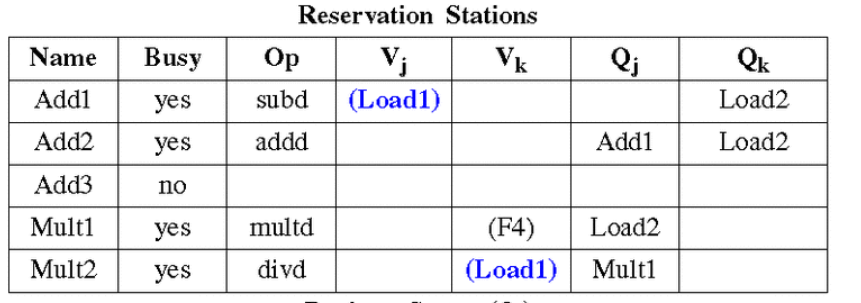
\includegraphics[scale=0.5]{pics/5-reservation-status.png}
        \caption{\lr{Reservation Status}}
        \label{pic:reservation_status}
    \end{figure}
    مرحله‌ی اول برای دستورات
    \lr{issue}
    هست. در این مرحله عملا ما دستور را به یکی از واحد‌های اجرایی
    \lr{CPU}
    می‌دهیم. به عنوان مثال اگر درخواست ضرب شده بود و یک واحد ضرب کننده خالی بود، به واحد ضرب کننده
    دستور را
    \emph{issue}
    می‌کنیم. اما در صورتی که واحد ضرب کننده‌ای خالی نبود باید اینقدر دستور را نگه داریم که یکی
    خالی شود.
    اما مشکل دیگری که می‌تواند به وجود آید این است که عملگر‌های دستور آماده نباشند. مثلا یک دستور
    \codeword{add}
    باید منتظر جواب یک دستور
    \codeword{mult}
    بماند. در این حالت باز نیست دستور را
    \lr{issue}
    می‌کنیم ولی از آنجا که مقدار واقعی رجیستر را نداریم،‌ در واحد محاسباتی باید صبر کنیم که مقدار
    آن مشخص شود.

    مرحله‌ی بعدی
    \lr{execute}
    است. در این مرحله اولین اتفاقی که می‌افتد این است که صبر می‌کند که تمامی ورودی‌های دستور آماده شوند.
    اگر دستور مربوط به مموری است،‌ در ابتدا آدرس درخواست شده را در
    \lr{reservation status table}
    مربوطه می‌ریزد و سپس منتظر می‌ماند که
    \lr{memory}
    آزاد شود. در صورتی که دستور مربوط به مموری نبود صرفا محاسبات را انجام می‌دهد.

    مرحله‌ی آخر
    \lr{write}
    است. در این مرحله در صورتی که دستور
    \codeword{store}
    بود که صرفا ذخیره سازه را انجام می‌دهیم. در غیر این صورت دیتای بدست آمده را بر روی
    \lr{CDB}
    می‌فرستیم.
    \lr{CDB} یا \lr{common data bus}
    یک باس مشترک بین تمامی
    \lr{PE}ها و \lr{reservation status table}
    است. زمانی که دیتای نتیجه بر روی باس گذاشته می‌شود در صورت نیاز
    \lr{PE}های
    دیگر این دیتا را بر می‌دارند و استفاده می‌کنند و یا اینکه در رجیستر فایل ذخیره می‌شود.

    برای رفع مشکلات
    \lr{dependency}
    از
    \lr{register renaming}
    استفاده می‌کنیم. در فاز
    \lr{stage}
    ما می‌توانیم متوجه شویم که آیا مقادیر درخواست شده در رجیسترفایل قرار دارند یا اینکه
    قرار است که از نتیجه‌ی دستور دیگری بیایند. به همین منظور اصلا نیازی به رجیستر فایل پیدا نمی‌کنیم در
    زمان خواندن!
    \item الگوریتم \lr{MP-Tomasulo} عملا بر روی توابع و نه دستور العمل‌ها موازی سازی را انجام می‌دهد.
    در ابتدا زمانی که برنامه کامپایل می‌شود گراف
    \lr{task dependency}
    کشیده می‌شود. این گراف نشان می‌دهد که هر کدام از
    \lr{task}ها
    چه جور وابستگی به
    \lr{task}های
    دیگر دارد. این وابستگی‌ها می‌توانند به صورت
    \lr{staic}
    موقع کامپایل کردن برنامه یا در زمان اجرا به کمک پردازنده‌ی
    \lr{scheduler}
    به کمک
    \lr{renaming}
    رفع شوند. برای نمونه می‌توانید به شکل شماره ۷ در مقاله مراجعه کنید.
    \item به نظر من یکی از بزرگترین نقاط قوت این الگوریتم این است که جاهایی که
    \lr{OoO}
    حتی در سخت افزار پشتیبانی نمی‌شود،‌ می‌توان این الگوریتم را استفاده کرد. چرا که این الگوریتم عملا
    بر روی
    \lr{task}ها
    زمان بندی را انجام می‌دهد و نه دستورات.

    برای نقاط ضعف به نظرم مشکل اجرا نشدن بهینه بر روی پردازنده‌ با تعداد هسته‌ی بالا مشکل بزرگتری تا
    \lr{FPGA}ها
    است. چرا که اکثر سیستم‌های امروزی و
    \lr{HPC}ها
    پردازنده‌هایی با تعداد هسته‌های بالا دارند.
    \item \begin{itemize}
        \item \lr{Reservation Stations}: مانند خود الگوریتم \lr{Tomasulo}
        صرفا برای
        \lr{function}ها
        ورودی‌ها،‌ خروجی‌ها،
        \lr{task} و\dots
        را نگه می‌دارد. در این جدول
        \lr{rename}
        کردن و حل کردن مشکلات
        \lr{WAW} و \lr{WAR}
        انجام می‌گیرد.
        \item \lr{The ReOrder Buffer (ROB)}: مثل \lr{ROB} داخل
        \lr{CPU}
        عمل می‌کند تا حدودی. چندین المان دارد مثل
        \lr{entry}،‌ \lr{busy}،‌ \lr{task}، \lr{dest} و \lr{value}.
        \item \lr{Function Unit Monitor and Arbitration}: وضعیت اجرای هر کدام از واحد‌های عملیاتی را زیر نظر دارد.
        این باعث می‌شود که بتوانیم
        \lr{load balancing}
        بر روی واحد‌‌های بیکار تر انجام دهیم.
    \end{itemize}
\end{enumerate}